\documentclass[12pt,a4paper]{article}

% incluyendo paquetes
\usepackage[utf8]{inputenc}
\usepackage[spanish]{babel}
\usepackage{milibreria}

\graphicspath{{C:/Users/HUAWEI/Pictures/imagesppt/}} %\incluye todos las imágenes de esa ruta
%\graphicspath{{D:/proyectos_latex/7mo_semestre/gestion_redes/informe_de_redes/main/images}}
\begin{document} % inicio  de documento 



\begin{titlepage}
    %\begin{tikzpicture}[overlay, remember picture]
    %    \fill[red] (10cm,-10cm) rectangle (5cm,-15cm);
    %\end{tikzpicture}
    
    \miRectangulo{-2cm}{-4cm}{2cm}{5cm}{rosado}
%   \miRectangulo{x     }{y }{x1    }{y1   }{color}
    
    \miRectangulo{-1.5cm}{-2cm}{-1.2cm}{23.5cm}{black} % 1
    \miRectangulo{-1.8cm}{23.5cm}{5.7cm}{23.2cm}{black} % 2
    \miRectangulo{5.025cm}{23.5cm}{5.33cm}{20cm}{black} % 3
    \miRectangulo{-2.7cm}{-1.7cm}{4.7cm}{-2cm}{black} % 4
    \miRectangulo{4.2cm}{-2cm}{4.5cm}{10cm}{black} % 5

    \begin{textblock}{100}(100,20)
        \begin{flushright}
        {\huge{\textbf{Universidad Nacional del Altiplano}}}\\
        {\normalsize{\textbf{Educando mentes, Cambiando el mundo}}}
        \end{flushright}
        
    \end{textblock}
    
    \begin{tikzpicture}[remember picture, overlay]
        \node at (current page.north west) [anchor=north west, xshift=120mm, yshift=-47mm] {\includegraphics[width=0.45\textwidth]{\logoright}};
    \end{tikzpicture}
    \begin{textblock}{100}(100,130)
        \begin{flushright}
            {\Large{\textbf{Facultad de Ingeniería Mecánica Eléctrica,
                    Electrónica y Sistemas}}}\\[10pt]
            {\large{\textbf{Escuela Profesional de Ingeniería\\ de Sistemas}}}
        \end{flushright}
    \end{textblock}

    \begin{textblock}{200}(10,163)
        \begin{center}
            
            %\textcolor{azul}{\rule{\linewidth}{0.80mm}}
            % titulo del articulo
            {\LARGE {\textbf{ Tipos de Auditoria }}} \par

            \textcolor{azul}{\rule{0.5\linewidth}{0.80mm}} \par
            \vspace{8mm}
            {\large{\textbf{ Auditoría en sistemas }}} \\[10pt]
            {\large{\textbf{\textcolor{azul}{ing. TICONA YANQUI FIDEL ERNESTO }}}} \\[20pt]
            {\large{\textbf{estudiante}}}\\[10pt]
            {\large{\textbf{$\looparrowright$   Larota Pilco David Brahyan  $\looparrowleft$ }}}\\[5pt]
            %{\large{\textbf{$\looparrowright$    Quispe Calcina Royer $\looparrowleft$ }}}\\[5pt]
            %{\large{\textbf{$\looparrowright$    Rojas Alejo Bruno $\looparrowleft$ }}}\\[5pt]
            %{\large{\textbf{$\looparrowright$  $\mathfrak{David\ Brahyan\ Larota\ Pilco}$   $\looparrowleft$ }}}\\[20pt]
            \today

        \end{center}
    \end{textblock}
\end{titlepage}
%//--------------------------------------
%@article{prueba,
%  title={prueba del documento lenguaje Latex},
%  author={Autor},
%  journal={https://www.overleaf.com/},
%  volume={13},
%  number={36},
%  pages={34--36},
%  year={2022}
%}
%
%
%\begin{figure}[h]
%    \centering
%    \includegraphics[width=0.5\textwidth]{images/medicion_con_tacometro.png}
%    \caption{se realizo la medición con el tacómetro} 
%\end{figure}
%
%\begin{tabular}{ l c l }
%Tipo  			& = & 	GL-90L-4B5 \\
%Ip              & = &	55 \\
%Cos  $\varphi$    & = &  	  0.78 \\
%Voltaje         & = &	 230/400V \\
%Potencia	    & = &	2HP \\
%Intensidad    	& = & 	6.1/3.5 \\
%Frecuencia  	& = & 	60HZ \\
%Rpm     		& = &	1680 
%\end{tabular} % incluyendo la caratula
%\tableofcontents % índice automático
\pagestyle{fancy} \mystyle \newpage % Aplicar el estilo de encabezado y pie de página
% inicio del documento  

\section{Introducción}
La simulación de estados de un proceso es una técnica que permite estudiar el comportamiento de un proceso en diferentes situaciones. En el contexto de la programación en C++, esta simulación se puede realizar utilizando exclusión mutua e hilos. La exclusión mutua garantiza que solo un hilo pueda acceder a un recurso compartido a la vez, evitando posibles problemas de concurrencia. Por otro lado, los hilos permiten ejecutar diferentes tareas de forma concurrente, lo que resulta especialmente útil para simular los diferentes estados de un proceso. En esta sección, se explorará el concepto de estados de un proceso y la importancia de simularlos en C++.

\section{Conceptos de Estados de un Proceso}
Los estados de un proceso son las diferentes etapas por las que puede pasar un programa en su ejecución. Estos estados incluyen el estado de "listo" cuando el proceso está preparado para ser ejecutado, el estado de "ejecución" cuando el proceso está utilizando la CPU para ejecutar sus instrucciones, y el estado de "bloqueado" cuando el proceso está esperando la finalización de una operación de entrada/salida. Comprender estos estados es fundamental para entender cómo funciona un programa y cómo se comporta durante su ejecución. En esta sección, se ahondará en el concepto de los estados de un proceso y su relevancia en la simulación en C++.
\begin{figure}[h]
    \centering
    \caption{Estados de un proceso} 
    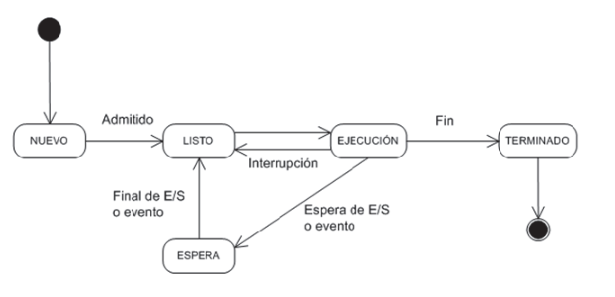
\includegraphics[width=0.7\textwidth]{images/estados.png}
    
\end{figure}

\newpage
\section{Arquitectura de como Simular}
Arquitectura del Modelo de Colas:
\begin{figure}[h]
    \centering
    \caption{Arquitectura del Modelo de Colas} 
    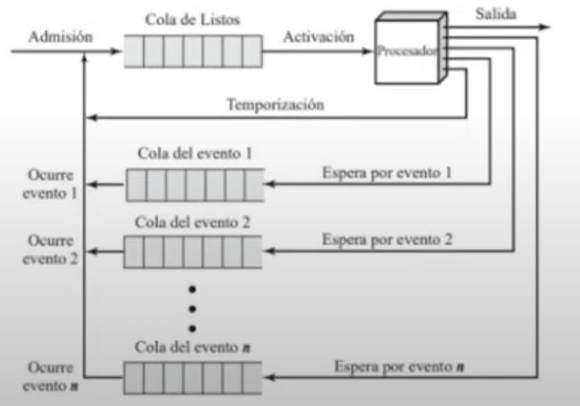
\includegraphics[width=0.7\textwidth]{images/procesos.png}
    
\end{figure}
Entonces tendremos una clase Proceso que tiene los siguientes atributos
\begin{lstlisting}
    
class Proceso
{
public:
	int identificador;
	estadoProceso estado;
    Matriz contador;
    Proceso() : identificador(ideProceso++), estado(NUEVO) {}

    Proceso(Matriz _cont) : identificador(ideProceso++), estado(NUEVO), contador(_cont) {}

};
\end{lstlisting}

Siguiente cada proceso tiene instrucciones, las instrucciones para la simulación será una matriz de nx3.
Donde n es la cantidad de instrucciones que tendrá el procesos, donde n = identificador de Introducción,
la matriz[n,0] = identificador del recurso a utilizar por ejemplo: I/O como memoria, micrófono, mouse, parlantes, impresora, etc.
por ultimo matriz[n,1] es el Tiempos de Ráfaga que el CPU le asigna a ese proceso, y por ultimo matriz[n,2] verifica si ese recurso ya ha sido ejecutado o no;
si esta en 0 o falso quiere decir que no ha sido ejecutado si esta en 1 o true ya ha sido ejecutado.

\begin{lstlisting}
    
    enum estadoProceso
{
    NUEVO,
    LISTO,
    EJECUCION,
    BLOQUEADO,
    TERMINADO
};

enum recursos
{
    teclado,
    camara,
    audio,
    mircrofono,
    impresora,
    disco_duro,
    memoria
};

class Matriz {
private:
    
public:
    int filas;
    int columnas;  
    int** matriz;
    Matriz(int filas = 1) : filas(filas), columnas(3) {
        matriz = new int* [filas];

        for (int i = 0; i < filas; ++i) {
            matriz[i] = new int[columnas];
            for (int j = 0; j < columnas; j++)
            {
                matriz[i][j] = 0;
            }
        }
    }

    int obtenerValor(int fila, int columna) {
        return matriz[fila][columna];
    }
    void establecerValor(int fila, int columna, int valor) {
        matriz[fila][columna] = valor;
    }
    void setMatriz(int** nuevaMatriz) {
        for (int i = 0; i < filas; ++i) {
            for (int j = 0; j < columnas; ++j) {
                matriz[i][j] = nuevaMatriz[i][j];
            }
        }
    }
    void imprimirMatriz() {
        for (int i = 0; i < filas; ++i) {
            for (int j = 0; j < columnas; ++j) {
                std::cout << matriz[i][j] << " ";
            }
            std::cout << std::endl;
        }
    }
};

    \end{lstlisting}
Luego procedemos a configurar el tiempo de simulación  cada 1 segundo
Asignamos valores:
\begin{lstlisting}
    
    void asignar()
{
    a.establecerValor(0, 0, impresora); // recurso a usar 
    a.establecerValor(0, 1, 2);        // tiempos de rafaga que nesecita

    a.establecerValor(1, 0, teclado);
    a.establecerValor(1, 1, 2);

    a.establecerValor(2, 0, camara);
    a.establecerValor(2, 1, 2);

    a.establecerValor(3, 0, mircrofono);
    a.establecerValor(3, 1, 2);

    a.establecerValor(4, 0, impresora);
    a.establecerValor(4, 1, 2);
    pa.contador = a; pa.estado = LISTO; sim.listos.push_back(pa);

    

    b.establecerValor(0, 0, teclado); // recurso a usar 
    b.establecerValor(0, 1, 20);        // tiempos de rafaga que nesecita

    b.establecerValor(1, 0, camara);
    b.establecerValor(1, 1, 50);

    b.establecerValor(2, 0, mircrofono);
    b.establecerValor(2, 1, 60);

    b.establecerValor(3, 0, disco_duro);
    b.establecerValor(3, 1, 80);

    b.establecerValor(4, 0, memoria);
    b.establecerValor(4, 1, 40);
    pb.contador = b; pb.estado = LISTO; sim.listos.push_back(pb);

    
    c.establecerValor(0, 0, memoria); // recurso a usar 
    c.establecerValor(0, 1, 20);        // tiempos de rafaga que nesecita

    c.establecerValor(1, 0, teclado);
    c.establecerValor(1, 1, 80);

    c.establecerValor(2, 0, camara);
    c.establecerValor(2, 1, 60);

    c.establecerValor(3, 0, disco_duro);
    c.establecerValor(3, 1, 20);

    c.establecerValor(4, 0, teclado);
    c.establecerValor(4, 1, 10);
    pc.contador = c; pc.estado = LISTO; sim.listos.push_back(pc);

    
    d.establecerValor(0, 0, audio); // recurso a usar 
    d.establecerValor(0, 1, 20);        // tiempos de rafaga que nesecita

    d.establecerValor(1, 0, teclado);
    d.establecerValor(1, 1, 10);

    d.establecerValor(2, 0, camara);
    d.establecerValor(2, 1, 60);

    d.establecerValor(3, 0, mircrofono);
    d.establecerValor(3, 1, 50);

    d.establecerValor(4, 0, impresora);
    d.establecerValor(4, 1, 10);
    pd.contador = d; pd.estado = LISTO; sim.listos.push_back(pd);


    e.establecerValor(0, 0, disco_duro); // recurso a usar 
    e.establecerValor(0, 1, 20);        // tiempos de rafaga que nesecita

    e.establecerValor(1, 0, memoria);
    e.establecerValor(1, 1, 40);

    e.establecerValor(2, 0, camara);
    e.establecerValor(2, 1, 60);

    e.establecerValor(3, 0, mircrofono);
    e.establecerValor(3, 1, 10);

    e.establecerValor(4, 0, audio);
    e.establecerValor(4, 1, 10);
    pe.contador = e; pe.estado = LISTO; sim.listos.push_back(pe);
    /*for (auto i = 0; i < sim.listos.size(); i++)
    {
        cout << sim.listos[i].identificador << endl;
    }*/
}
    \end{lstlisting}
\cite{prueba}
\newpage
\section{Referencias}
\bibliographystyle{apacite}
\bibliography{referencias.bib}


\end{document}